\section{Reproducibility}
\label{app:repro}

\paragraph{Artifacts.} Every table, plot and number in the paper is written by
\texttt{uv run cer p17-tables} from the committed artifacts of Phase~17 (\texttt{data/phase17/}) and,
read-only, the outcome files of Phases~9, 10, 14, 15 and~16. The generated files are committed under
\texttt{docs/paper/tables} and \texttt{docs/paper/figures}; each macro in \texttt{numbers.tex}
carries its artifact path, the SHA-256 prefix of that file and the JSON key it was read from.
Table~\ref{tab:sha} gives the full SHA-256 of the files the text cites; the Phase~9, 10 and 14 outcome files are
not in git, so their digests are the record.

\begin{table*}[t]
\centering
\scriptsize
\caption{SHA-256 of the artifacts the paper reads (written from the files by the generator).}
\label{tab:sha}
\begin{tabular}{ll}
\toprule
Artifact & SHA-256 \\
\midrule
\texttt{data/phase17/outcome.json} & \texttt{\shaOutcome} \\
\texttt{data/phase17/metrics.json} & \texttt{\shaMetrics} \\
\texttt{data/phase17/pool.json} & \texttt{\shaPool} \\
\texttt{data/phase17/integrity.json} & \texttt{\shaIntegrity} \\
\texttt{data/phase17/scoring-light.json} & \texttt{\shaScoringLight} \\
\texttt{data/phase17/scoring-strong.json} & \texttt{\shaScoringStrong} \\
\texttt{data/phase17/scoring-decision.json} & \texttt{\shaScoringDecision} \\
\texttt{data/phase17/published-figures.json} & \texttt{\shaPublished} \\
\texttt{data/phase9/outcome.json} & \texttt{\shaPhaseNineOutcome} \\
\texttt{data/phase10/outcome.json} & \texttt{\shaPhaseTenOutcome} \\
\texttt{data/phase14/outcome.json} & \texttt{\shaPhaseFourteenOutcome} \\
\texttt{data/phase15/outcome.json} & \texttt{\shaPhaseFifteenOutcome} \\
\texttt{data/phase16/outcome.json} & \texttt{\shaPhaseSixteenOutcome} \\
\bottomrule
\end{tabular}
\end{table*}

\paragraph{Pins.} Table~\ref{tab:judges} gives each judge's model, revision, parameters, maximum
length and precision; each scoring manifest also records the library versions, the code commit,
the weights' SHA-256 and the serving command. The extractor is GLiNER
GLiNER (the medium zero-shot model) at a pinned revision recorded in the repository's
configuration, and the Dense model is BGE-small at a pinned revision. Seeds are explicit and ties are broken by a deterministic rule.

\paragraph{The rented session.} All scoring ran in one session on a rented RTX~4090 at
\judgeRateLight{} USD per hour, driven over SSH from the laptop: \sessionHours{} h \sessionMinutes{} min, a balance
drop of \usdSession{} USD, of which \usdGpuAttributable{} USD is attributable to scoring (derived from
measured time and the hourly rate; Table~\ref{tab:judgecost}). Nothing else ran on a GPU in this
phase; the paper itself builds on a laptop.

\paragraph{Build.} \texttt{uv run python docs/paper/build.py} regenerates the tables, runs Tectonic
on \texttt{docs/paper/main.tex}, and prints the page count and the SHA-256 of the PDF. The
\texttt{\textbackslash anonymoustrue} switch in \texttt{main.tex} drops the author, the repository
URL and the acknowledgements for double-blind review. The R5 guard
(\texttt{paper.r5\_violations}) runs inside \texttt{cer p17-tables} and refuses any hand-written
number with a decimal point, a thousands separator or a percent sign.

\section{Paired comparisons (D5)}
\label{app:d5}

\begin{table*}[t]
\centering
\scriptsize
\caption{\capDFiveHotpotqa}
% Generated by `cer p17-tables`; do not edit.
% caption: HotpotQA dev, 7,405 questions: the paired comparisons of D5 (exact two-sided McNemar on Full Support); the label is that of J(P14) against J(P10-B).
\begin{tabular}{lrrrrrl}
\toprule
Comparison & Wins & Losses & Ties & Delta (pp) & p & Label \\
\midrule
J-light(P10-A) vs P10-A & 665 & 228 & 6,512 & +5.90 & $3.0\times10^{-50}$ &  \\
J-light(P10-B) vs P10-B & 445 & 251 & 6,709 & +2.62 & $1.8\times10^{-13}$ &  \\
J-light(P10-C) vs P10-C & 524 & 411 & 6,470 & +1.53 & $2.5\times10^{-4}$ &  \\
J-light(P14) vs J-light(P10-B) & 383 & 59 & 6,963 & +4.38 & $3.1\times10^{-59}$ & HOP\_ADDS\_UNDER\_JUDGE \\
J-light(P14) vs P14 & 441 & 611 & 6,353 & $-$2.30 & $1.8\times10^{-7}$ &  \\
\midrule
J-strong(P10-A) vs P10-A & 875 & 36 & 6,494 & +11.33 & $5.6\times10^{-210}$ &  \\
J-strong(P10-B) vs P10-B & 685 & 23 & 6,697 & +8.94 & $1.5\times10^{-170}$ &  \\
J-strong(P10-C) vs P10-C & 846 & 78 & 6,481 & +10.37 & $1.0\times10^{-163}$ &  \\
J-strong(P14) vs J-strong(P10-B) & 780 & 67 & 6,558 & +9.63 & $6.4\times10^{-155}$ & HOP\_ADDS\_UNDER\_JUDGE \\
J-strong(P14) vs P14 & 798 & 111 & 6,496 & +9.28 & $6.9\times10^{-129}$ &  \\
\midrule
J-decision(P10-A) vs P10-A & 182 & 2,749 & 4,474 & $-$34.67 & $<10^{-300}$ &  \\
J-decision(P10-B) vs P10-B & 148 & 2,802 & 4,455 & $-$35.84 & $<10^{-300}$ &  \\
J-decision(P10-C) vs P10-C & 194 & 3,012 & 4,199 & $-$38.06 & $<10^{-300}$ &  \\
J-decision(P14) vs J-decision(P10-B) & 264 & 256 & 6,885 & +0.11 & $7.6\times10^{-1}$ & HOP\_NEUTRAL\_UNDER\_JUDGE \\
J-decision(P14) vs P14 & 155 & 3,489 & 3,761 & $-$45.02 & $<10^{-300}$ &  \\
\midrule
J-decision(P10-B) vs J-strong(P10-B) & 12 & 3,328 & 4,065 & $-$44.78 & $<10^{-300}$ &  \\
J-strong(P10-B) vs J-light(P10-B) & 494 & 26 & 6,885 & +6.32 & $3.3\times10^{-113}$ &  \\
\bottomrule
\end{tabular}

\end{table*}

\begin{table*}[t]
\centering
\scriptsize
\caption{\capDFiveMusique}
% Generated by `cer p17-tables`; do not edit.
% caption: MuSiQue validation, 2,417 questions: the paired comparisons of D5 (exact two-sided McNemar on Full Support); the label is that of J(P14) against J(P10-B).
\begin{tabular}{lrrrrrl}
\toprule
Comparison & Wins & Losses & Ties & Delta (pp) & p & Label \\
\midrule
J-light(P10-A) vs P10-A & 201 & 42 & 2,174 & +6.58 & $4.6\times10^{-26}$ &  \\
J-light(P10-B) vs P10-B & 176 & 56 & 2,185 & +4.96 & $1.2\times10^{-15}$ &  \\
J-light(P10-C) vs P10-C & 173 & 172 & 2,072 & +0.04 & $1.0\times10^{0}$ &  \\
J-light(P14) vs J-light(P10-B) & 68 & 15 & 2,334 & +2.19 & $3.2\times10^{-9}$ & HOP\_ADDS\_UNDER\_JUDGE \\
J-light(P14) vs P14 & 172 & 236 & 2,009 & $-$2.65 & $1.8\times10^{-3}$ &  \\
\midrule
J-strong(P10-A) vs P10-A & 247 & 41 & 2,129 & +8.52 & $4.9\times10^{-37}$ &  \\
J-strong(P10-B) vs P10-B & 230 & 50 & 2,137 & +7.45 & $9.3\times10^{-29}$ &  \\
J-strong(P10-C) vs P10-C & 261 & 126 & 2,030 & +5.59 & $5.9\times10^{-12}$ &  \\
J-strong(P14) vs J-strong(P10-B) & 190 & 23 & 2,204 & +6.91 & $7.0\times10^{-34}$ & HOP\_ADDS\_UNDER\_JUDGE \\
J-strong(P14) vs P14 & 272 & 162 & 1,983 & +4.55 & $1.4\times10^{-7}$ &  \\
\midrule
J-decision(P10-A) vs P10-A & 56 & 337 & 2,024 & $-$11.63 & $5.3\times10^{-50}$ &  \\
J-decision(P10-B) vs P10-B & 47 & 397 & 1,973 & $-$14.48 & $4.1\times10^{-70}$ &  \\
J-decision(P10-C) vs P10-C & 56 & 504 & 1,857 & $-$18.54 & $3.9\times10^{-91}$ &  \\
J-decision(P14) vs J-decision(P10-B) & 70 & 22 & 2,325 & +1.99 & $5.3\times10^{-7}$ & HOP\_ADDS\_UNDER\_JUDGE \\
J-decision(P14) vs P14 & 42 & 581 & 1,794 & $-$22.30 & $2.5\times10^{-122}$ &  \\
\midrule
J-decision(P10-B) vs J-strong(P10-B) & 22 & 552 & 1,843 & $-$21.93 & $9.9\times10^{-134}$ &  \\
J-strong(P10-B) vs J-light(P10-B) & 121 & 61 & 2,235 & +2.48 & $1.0\times10^{-5}$ &  \\
\bottomrule
\end{tabular}

\end{table*}

\begin{table*}[t]
\centering
\scriptsize
\caption{\capDFiveMultihopRag}
% Generated by `cer p17-tables`; do not edit.
% caption: MultiHop-RAG answerable, 2,255 questions: the paired comparisons of D5 (exact two-sided McNemar on Full Support); the label is that of J(P14) against J(P10-B).
\begin{tabular}{lrrrrrl}
\toprule
Comparison & Wins & Losses & Ties & Delta (pp) & p & Label \\
\midrule
J-light(P10-A) vs P10-A & 124 & 152 & 1,979 & $-$1.24 & $1.0\times10^{-1}$ &  \\
J-light(P10-B) vs P10-B & 89 & 324 & 1,842 & $-$10.42 & $1.9\times10^{-32}$ &  \\
J-light(P10-C) vs P10-C & 105 & 283 & 1,867 & $-$7.89 & $5.6\times10^{-20}$ &  \\
J-light(P14) vs J-light(P10-B) & 14 & 27 & 2,214 & $-$0.58 & $6.0\times10^{-2}$ & HOP\_NEUTRAL\_UNDER\_JUDGE \\
J-light(P14) vs P14 & 98 & 272 & 1,885 & $-$7.72 & $4.7\times10^{-20}$ &  \\
\midrule
J-strong(P10-A) vs P10-A & 313 & 38 & 1,904 & +12.20 & $6.2\times10^{-55}$ &  \\
J-strong(P10-B) vs P10-B & 289 & 54 & 1,912 & +10.42 & $5.8\times10^{-40}$ &  \\
J-strong(P10-C) vs P10-C & 321 & 50 & 1,884 & +12.02 & $1.5\times10^{-49}$ &  \\
J-strong(P14) vs J-strong(P10-B) & 24 & 49 & 2,182 & $-$1.11 & $4.6\times10^{-3}$ & HOP\_HURTS\_UNDER\_JUDGE \\
J-strong(P14) vs P14 & 338 & 54 & 1,863 & +12.59 & $2.4\times10^{-51}$ &  \\
\midrule
J-decision(P10-A) vs P10-A & 80 & 251 & 1,924 & $-$7.58 & $1.1\times10^{-21}$ &  \\
J-decision(P10-B) vs P10-B & 60 & 439 & 1,756 & $-$16.81 & $3.2\times10^{-72}$ &  \\
J-decision(P10-C) vs P10-C & 59 & 407 & 1,789 & $-$15.43 & $5.2\times10^{-65}$ &  \\
J-decision(P14) vs J-decision(P10-B) & 21 & 44 & 2,190 & $-$1.02 & $5.9\times10^{-3}$ & HOP\_HURTS\_UNDER\_JUDGE \\
J-decision(P14) vs P14 & 71 & 399 & 1,785 & $-$14.55 & $1.9\times10^{-56}$ &  \\
\midrule
J-decision(P10-B) vs J-strong(P10-B) & 26 & 640 & 1,589 & $-$27.23 & $2.6\times10^{-154}$ &  \\
J-strong(P10-B) vs J-light(P10-B) & 511 & 41 & 1,703 & +20.84 & $2.5\times10^{-104}$ &  \\
\bottomrule
\end{tabular}

\end{table*}

\section{Comparable metrics (D6)}
\label{app:d6}

\begin{table*}[t]
\centering
\scriptsize
\caption{\capDSixHotpotqa}
\pagetable{tables/d6-hotpotqa}
\end{table*}

\begin{table*}[t]
\centering
\scriptsize
\caption{\capDSixMusique}
\pagetable{tables/d6-musique}
\end{table*}

\begin{table*}[t]
\centering
\scriptsize
\caption{\capDSixMultihopRag}
\pagetable{tables/d6-multihop-rag}
\end{table*}

\section{Budget curves and ceilings}
\label{app:more}

\begin{table}[t]
\centering
\scriptsize
\caption{\capBudgetCurve}
\coltable{tables/budget-curve}
\end{table}

\begin{figure}[t]
\centering
% Generated by `cer p17-tables`; do not edit. Coordinates are written from the artifacts.
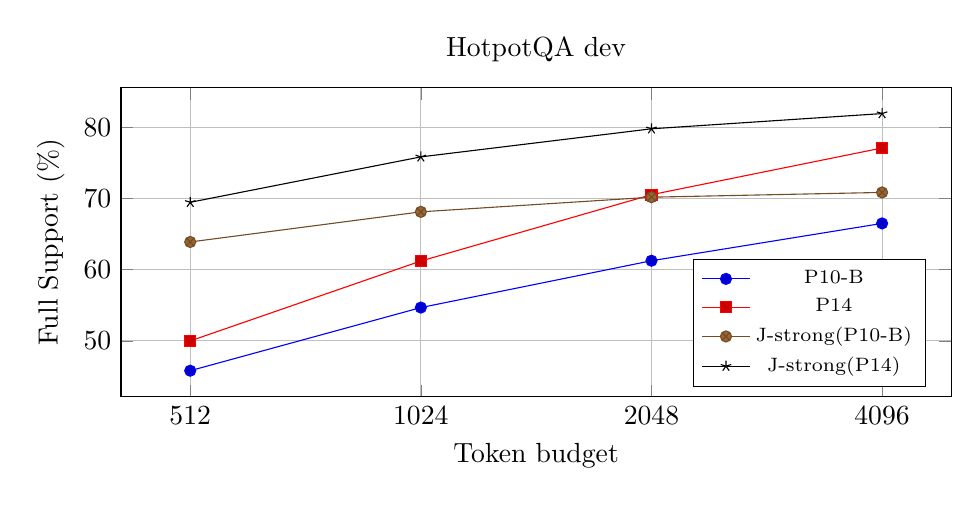
\begin{tikzpicture}
\begin{axis}[width=\columnwidth, height=5.5cm, xmode=log, log basis x=2, xtick={512,1024,2048,4096}, xticklabels={512,1024,2048,4096}, xlabel={Token budget}, ylabel={Full Support (\%)}, grid=major, legend pos=south east, legend style={font=\scriptsize}, title={HotpotQA dev}]
\addplot coordinates {(512,45.79) (1024,54.67) (2048,61.26) (4096,66.51)};
\addlegendentry{P10-B}
\addplot coordinates {(512,49.98) (1024,61.22) (2048,70.55) (4096,77.12)};
\addlegendentry{P14}
\addplot coordinates {(512,63.90) (1024,68.14) (2048,70.20) (4096,70.87)};
\addlegendentry{J-strong(P10-B)}
\addplot coordinates {(512,69.48) (1024,75.87) (2048,79.82) (4096,81.96)};
\addlegendentry{J-strong(P14)}
\end{axis}
\end{tikzpicture}

\caption{\FS{} against the token budget on HotpotQA development questions, for P10-B and P14
with and without J-strong.}
\end{figure}

\begin{figure}[t]
\centering
% Generated by `cer p17-tables`; do not edit. Coordinates are written from the artifacts.
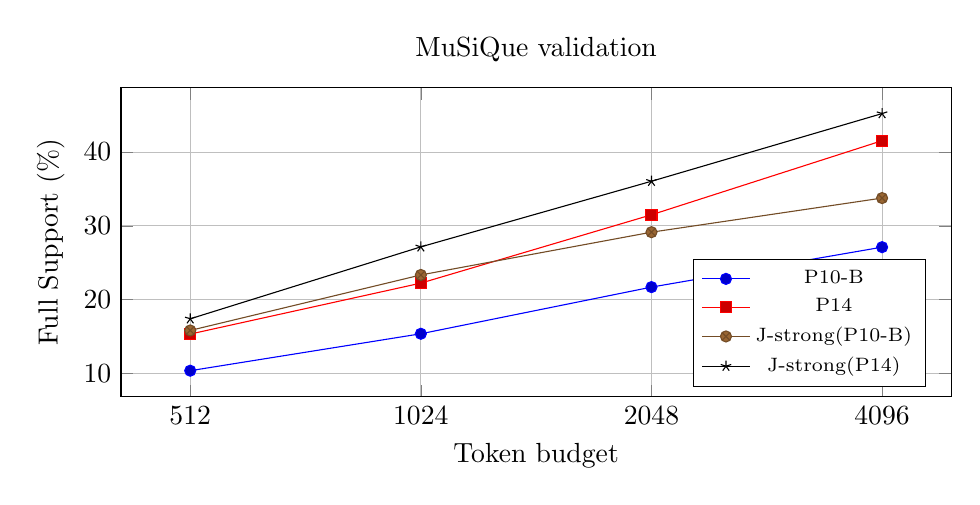
\begin{tikzpicture}
\begin{axis}[width=\columnwidth, height=5.5cm, xmode=log, log basis x=2, xtick={512,1024,2048,4096}, xticklabels={512,1024,2048,4096}, xlabel={Token budget}, ylabel={Full Support (\%)}, grid=major, legend pos=south east, legend style={font=\scriptsize}, title={MuSiQue validation}]
\addplot coordinates {(512,10.34) (1024,15.35) (2048,21.68) (4096,27.10)};
\addlegendentry{P10-B}
\addplot coordinates {(512,15.31) (1024,22.22) (2048,31.49) (4096,41.54)};
\addlegendentry{P14}
\addplot coordinates {(512,15.80) (1024,23.33) (2048,29.13) (4096,33.76)};
\addlegendentry{J-strong(P10-B)}
\addplot coordinates {(512,17.38) (1024,27.14) (2048,36.04) (4096,45.22)};
\addlegendentry{J-strong(P14)}
\end{axis}
\end{tikzpicture}

\caption{The same on MuSiQue validation.}
\end{figure}

\begin{figure}[t]
\centering
% Generated by `cer p17-tables`; do not edit. Coordinates are written from the artifacts.
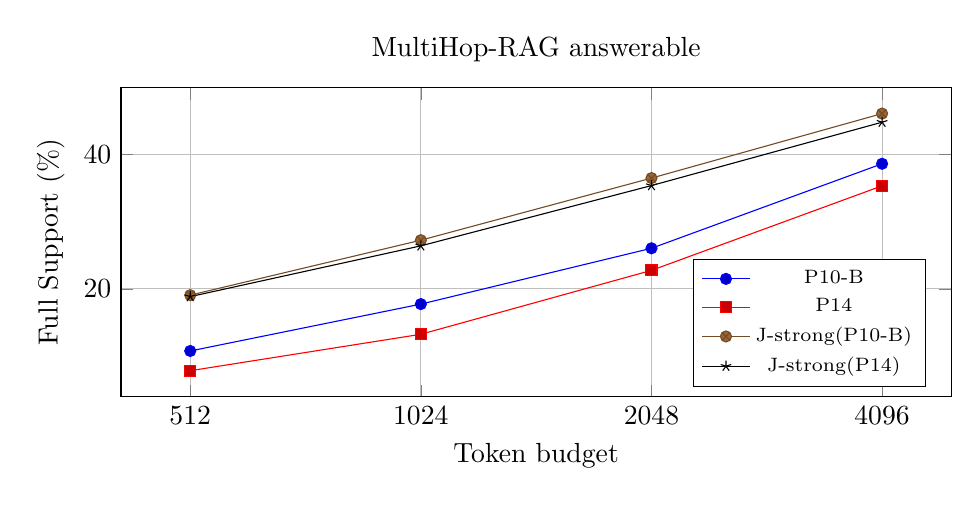
\begin{tikzpicture}
\begin{axis}[width=\columnwidth, height=5.5cm, xmode=log, log basis x=2, xtick={512,1024,2048,4096}, xticklabels={512,1024,2048,4096}, xlabel={Token budget}, ylabel={Full Support (\%)}, grid=major, legend pos=south east, legend style={font=\scriptsize}, title={MultiHop-RAG answerable}]
\addplot coordinates {(512,10.78) (1024,17.74) (2048,26.03) (4096,38.58)};
\addlegendentry{P10-B}
\addplot coordinates {(512,7.85) (1024,13.26) (2048,22.75) (4096,35.30)};
\addlegendentry{P14}
\addplot coordinates {(512,19.07) (1024,27.23) (2048,36.45) (4096,46.03)};
\addlegendentry{J-strong(P10-B)}
\addplot coordinates {(512,18.85) (1024,26.39) (2048,35.34) (4096,44.75)};
\addlegendentry{J-strong(P14)}
\end{axis}
\end{tikzpicture}

\caption{The same on MultiHop-RAG.}
\end{figure}

\begin{table*}[t]
\centering
\scriptsize
\caption{\capCeiling}
\pagetable{tables/ceiling}
\end{table*}

\clearpage
\onecolumn
\section{Published figures, row by row}
\label{app:pub}

\begingroup
\scriptsize
\setlength{\tabcolsep}{3pt}
% Generated by `cer p17-tables`; do not edit.
% caption: HotpotQA: published figures, not a paired comparison. Each row was read in the paper itself; the last column says what differs from our setting.
\begin{tabular}{p{2.4cm}p{2.0cm}rrp{2.6cm}p{1.6cm}p{5.2cm}l}
\toprule
System & Metric & Value & Questions & Corpus & Training or LLM & Differences from ours & Source \\
\midrule
BM25 & nDCG@10 & 0.603 & 7,405 & HotpotQA Wikipedia abstracts (BEIR cut) (5,233,329) & none & Same 7,405 questions and 5,233,329 paragraphs as our fullwiki setting, but the metric is nDCG@10 over graded-binary per-paragraph relevance, not Full Support @2,048 tokens nor paragraph-pair recall at k; the BEIR split is the official 7,405-question set, which we use as dev. Lexical, no training. & \cite{thakur2021beir} \\
BM25 + cross-encoder reranking (MiniLM-L6, top-100) & nDCG@10 & 0.707 & 7,405 & HotpotQA Wikipedia abstracts (BEIR cut) (5,233,329) & trained retriever & Same 7,405 questions and 5,233,329 paragraphs as our fullwiki setting, but the metric is nDCG@10 over graded-binary per-paragraph relevance, not Full Support @2,048 tokens nor paragraph-pair recall at k; the BEIR split is the official 7,405-question set, which we use as dev. First stage BM25 (Anserini), top-100 reranked by a 6-layer 384-d MiniLM cross-encoder trained on MS MARCO (zero-shot on HotpotQA); the closest published analogue of our J-light recipe, though our rerank depth and unit differ. & \cite{thakur2021beir} \\
DPR & nDCG@10 & 0.391 & 7,405 & HotpotQA Wikipedia abstracts (BEIR cut) (5,233,329) & trained retriever & Same 7,405 questions and 5,233,329 paragraphs as our fullwiki setting, but the metric is nDCG@10 over graded-binary per-paragraph relevance, not Full Support @2,048 tokens nor paragraph-pair recall at k; the BEIR split is the official 7,405-question set, which we use as dev. Trained on MS MARCO (BEIR re-trained it), zero-shot on HotpotQA. & \cite{thakur2021beir} \\
ANCE & nDCG@10 & 0.456 & 7,405 & HotpotQA Wikipedia abstracts (BEIR cut) (5,233,329) & trained retriever & Same 7,405 questions and 5,233,329 paragraphs as our fullwiki setting, but the metric is nDCG@10 over graded-binary per-paragraph relevance, not Full Support @2,048 tokens nor paragraph-pair recall at k; the BEIR split is the official 7,405-question set, which we use as dev. Trained on MS MARCO, zero-shot on HotpotQA. & \cite{thakur2021beir} \\
TAS-B & nDCG@10 & 0.584 & 7,405 & HotpotQA Wikipedia abstracts (BEIR cut) (5,233,329) & trained retriever & Same 7,405 questions and 5,233,329 paragraphs as our fullwiki setting, but the metric is nDCG@10 over graded-binary per-paragraph relevance, not Full Support @2,048 tokens nor paragraph-pair recall at k; the BEIR split is the official 7,405-question set, which we use as dev. Trained on MS MARCO, zero-shot on HotpotQA. & \cite{thakur2021beir} \\
ColBERT (late interaction, end-to-end) & nDCG@10 & 0.593 & 7,405 & HotpotQA Wikipedia abstracts (BEIR cut) (5,233,329) & trained retriever & Same 7,405 questions and 5,233,329 paragraphs as our fullwiki setting, but the metric is nDCG@10 over graded-binary per-paragraph relevance, not Full Support @2,048 tokens nor paragraph-pair recall at k; the BEIR split is the official 7,405-question set, which we use as dev. Trained on MS MARCO, zero-shot on HotpotQA. & \cite{thakur2021beir} \\
MDR (multi-hop dense retriever, trained on HotpotQA) & R@2 (recall at k retrieved passages, percent) & 65.9 & -- & HotpotQA fullwiki Wikipedia (the paper does not state a size in the sections read; Baleen Appendix A describes the shared corpus as about 5M first paragraphs) & trained retriever & Trained on HotpotQA train with a hyperlink-free two-hop dense retriever; recall at k paragraphs, not Full Support @2,048 tokens. The dev question count is not stated in the sections read. Baleen (footnote 2) describes this style of metric as both gold passages within the top k, and reports 82.9 for MDR P-R@20 from the authors' released retrieval versus the 80.2 above. & \cite{xiong2021mdr} \\
MDR (multi-hop dense retriever, trained on HotpotQA) & R@10 (recall at k retrieved passages, percent) & 77.5 & -- & HotpotQA fullwiki Wikipedia (the paper does not state a size in the sections read; Baleen Appendix A describes the shared corpus as about 5M first paragraphs) & trained retriever & Trained on HotpotQA train with a hyperlink-free two-hop dense retriever; recall at k paragraphs, not Full Support @2,048 tokens. The dev question count is not stated in the sections read. Baleen (footnote 2) describes this style of metric as both gold passages within the top k, and reports 82.9 for MDR P-R@20 from the authors' released retrieval versus the 80.2 above. & \cite{xiong2021mdr} \\
MDR (multi-hop dense retriever, trained on HotpotQA) & R@20 (recall at k retrieved passages, percent) & 80.2 & -- & HotpotQA fullwiki Wikipedia (the paper does not state a size in the sections read; Baleen Appendix A describes the shared corpus as about 5M first paragraphs) & trained retriever & Trained on HotpotQA train with a hyperlink-free two-hop dense retriever; recall at k paragraphs, not Full Support @2,048 tokens. The dev question count is not stated in the sections read. Baleen (footnote 2) describes this style of metric as both gold passages within the top k, and reports 82.9 for MDR P-R@20 from the authors' released retrieval versus the 80.2 above. & \cite{xiong2021mdr} \\
Baleen (FLIPR + condenser, trained on HotpotQA) & P-EM (both gold passages exactly selected, percent) & 86.7 & 7,405 & Wikipedia dump of Oct 2017 released by Yang et al. (first paragraph of each page) (5,000,000) & trained retriever & Trained multi-hop retriever with a condensing stage; P-EM is exact match of the final selected pair, a different metric from Full Support @2,048 tokens. corpus\_size is the paper's own 'approximately 5M passages'. & \cite{khattab2021baleen} \\
Baleen (FLIPR + condenser, trained on HotpotQA) & P-R@20 (top-20 passages contain both gold passages, percent) & 93.3 & 7,405 & Wikipedia dump of Oct 2017 released by Yang et al. (first paragraph of each page) (5,000,000) & trained retriever & Top-20 is the union of the top 10 of hop one and the top 10 of hop two; trained retriever; paragraph-count budget, not a token budget. corpus\_size is the paper's 'approximately 5M passages'. & \cite{khattab2021baleen} \\
BM25 & passage recall@2 (percent) on HotpotQA & 55.4 & 1,000 & HotpotQA: gold and distractor passages of the 1,000 questions (IRCoT-style pooled corpus) (9,221) & none & Not our setting: a 1,000-question subset of the validation set, and a small per-benchmark pooled corpus built from the gold and distractor passages of those questions (not the full Wikipedia); passage recall at 2 or 5, not Full Support @2,048 tokens. Lexical baseline. & \cite{gutierrez2024hipporag} \\
BM25 & passage recall@5 (percent) on HotpotQA & 72.2 & 1,000 & HotpotQA: gold and distractor passages of the 1,000 questions (IRCoT-style pooled corpus) (9,221) & none & Not our setting: a 1,000-question subset of the validation set, and a small per-benchmark pooled corpus built from the gold and distractor passages of those questions (not the full Wikipedia); passage recall at 2 or 5, not Full Support @2,048 tokens. Lexical baseline. & \cite{gutierrez2024hipporag} \\
ColBERTv2 & passage recall@2 (percent) on HotpotQA & 64.7 & 1,000 & HotpotQA: gold and distractor passages of the 1,000 questions (IRCoT-style pooled corpus) (9,221) & trained retriever & Not our setting: a 1,000-question subset of the validation set, and a small per-benchmark pooled corpus built from the gold and distractor passages of those questions (not the full Wikipedia); passage recall at 2 or 5, not Full Support @2,048 tokens. Trained retriever (ColBERTv2), single step. & \cite{gutierrez2024hipporag} \\
ColBERTv2 & passage recall@5 (percent) on HotpotQA & 79.3 & 1,000 & HotpotQA: gold and distractor passages of the 1,000 questions (IRCoT-style pooled corpus) (9,221) & trained retriever & Not our setting: a 1,000-question subset of the validation set, and a small per-benchmark pooled corpus built from the gold and distractor passages of those questions (not the full Wikipedia); passage recall at 2 or 5, not Full Support @2,048 tokens. Trained retriever (ColBERTv2), single step. & \cite{gutierrez2024hipporag} \\
HippoRAG (ColBERTv2) & passage recall@2 (percent) on HotpotQA & 60.5 & 1,000 & HotpotQA: gold and distractor passages of the 1,000 questions (IRCoT-style pooled corpus) (9,221) & LLM in the loop & Not our setting: a 1,000-question subset of the validation set, and a small per-benchmark pooled corpus built from the gold and distractor passages of those questions (not the full Wikipedia); passage recall at 2 or 5, not Full Support @2,048 tokens. Uses GPT-3.5-turbo for OpenIE indexing and a knowledge-graph Personalized PageRank at query time over ColBERTv2 retrieval. & \cite{gutierrez2024hipporag} \\
HippoRAG (ColBERTv2) & passage recall@5 (percent) on HotpotQA & 77.7 & 1,000 & HotpotQA: gold and distractor passages of the 1,000 questions (IRCoT-style pooled corpus) (9,221) & LLM in the loop & Not our setting: a 1,000-question subset of the validation set, and a small per-benchmark pooled corpus built from the gold and distractor passages of those questions (not the full Wikipedia); passage recall at 2 or 5, not Full Support @2,048 tokens. Uses GPT-3.5-turbo for OpenIE indexing and a knowledge-graph Personalized PageRank at query time over ColBERTv2 retrieval. & \cite{gutierrez2024hipporag} \\
IRCoT + ColBERTv2 & passage recall@2 (percent) on HotpotQA & 67.9 & 1,000 & HotpotQA: gold and distractor passages of the 1,000 questions (IRCoT-style pooled corpus) (9,221) & LLM in the loop & Not our setting: a 1,000-question subset of the validation set, and a small per-benchmark pooled corpus built from the gold and distractor passages of those questions (not the full Wikipedia); passage recall at 2 or 5, not Full Support @2,048 tokens. IRCoT interleaves ColBERTv2 retrieval with LLM chain-of-thought (GPT-3.5) at query time. & \cite{gutierrez2024hipporag} \\
IRCoT + ColBERTv2 & passage recall@5 (percent) on HotpotQA & 82 & 1,000 & HotpotQA: gold and distractor passages of the 1,000 questions (IRCoT-style pooled corpus) (9,221) & LLM in the loop & Not our setting: a 1,000-question subset of the validation set, and a small per-benchmark pooled corpus built from the gold and distractor passages of those questions (not the full Wikipedia); passage recall at 2 or 5, not Full Support @2,048 tokens. IRCoT interleaves ColBERTv2 retrieval with LLM chain-of-thought (GPT-3.5) at query time. & \cite{gutierrez2024hipporag} \\
IRCoT + HippoRAG (ColBERTv2) & passage recall@2 (percent) on HotpotQA & 67 & 1,000 & HotpotQA: gold and distractor passages of the 1,000 questions (IRCoT-style pooled corpus) (9,221) & LLM in the loop & Not our setting: a 1,000-question subset of the validation set, and a small per-benchmark pooled corpus built from the gold and distractor passages of those questions (not the full Wikipedia); passage recall at 2 or 5, not Full Support @2,048 tokens. LLM chain-of-thought at query time plus an LLM-built knowledge graph. & \cite{gutierrez2024hipporag} \\
IRCoT + HippoRAG (ColBERTv2) & passage recall@5 (percent) on HotpotQA & 83 & 1,000 & HotpotQA: gold and distractor passages of the 1,000 questions (IRCoT-style pooled corpus) (9,221) & LLM in the loop & Not our setting: a 1,000-question subset of the validation set, and a small per-benchmark pooled corpus built from the gold and distractor passages of those questions (not the full Wikipedia); passage recall at 2 or 5, not Full Support @2,048 tokens. LLM chain-of-thought at query time plus an LLM-built knowledge graph. & \cite{gutierrez2024hipporag} \\
BM25 & passage recall@2 (percent) on HotpotQA & 57.3 & 1,000 & HotpotQA: pooled passages of the 1,000 sampled questions (9,811) & none & Not our setting: a 1,000-question sample of the validation set, and a small per-benchmark pooled corpus built from the gold and distractor passages of those questions (not the full Wikipedia); passage recall at 2 or 5, not Full Support @2,048 tokens. Lexical baseline, reported in the HippoRAG 2 paper's own table. & \cite{gutierrez2025hipporag2} \\
BM25 & passage recall@5 (percent) on HotpotQA & 74.8 & 1,000 & HotpotQA: pooled passages of the 1,000 sampled questions (9,811) & none & Not our setting: a 1,000-question sample of the validation set, and a small per-benchmark pooled corpus built from the gold and distractor passages of those questions (not the full Wikipedia); passage recall at 2 or 5, not Full Support @2,048 tokens. Lexical baseline, reported in the HippoRAG 2 paper's own table. & \cite{gutierrez2025hipporag2} \\
NV-Embed-v2 (7B dense retriever) & passage recall@2 (percent) on HotpotQA & 84.1 & 1,000 & HotpotQA: pooled passages of the 1,000 sampled questions (9,811) & trained retriever & Not our setting: a 1,000-question sample of the validation set, and a small per-benchmark pooled corpus built from the gold and distractor passages of those questions (not the full Wikipedia); passage recall at 2 or 5, not Full Support @2,048 tokens. A 7B dense embedding model, far larger than our BGE-small; no LLM at query time. & \cite{gutierrez2025hipporag2} \\
NV-Embed-v2 (7B dense retriever) & passage recall@5 (percent) on HotpotQA & 94.5 & 1,000 & HotpotQA: pooled passages of the 1,000 sampled questions (9,811) & trained retriever & Not our setting: a 1,000-question sample of the validation set, and a small per-benchmark pooled corpus built from the gold and distractor passages of those questions (not the full Wikipedia); passage recall at 2 or 5, not Full Support @2,048 tokens. A 7B dense embedding model, far larger than our BGE-small; no LLM at query time. & \cite{gutierrez2025hipporag2} \\
HippoRAG 2 (Llama-3.3-70B-Instruct) & passage recall@2 (percent) on HotpotQA & 83.5 & 1,000 & HotpotQA: pooled passages of the 1,000 sampled questions (9,811) & LLM in the loop & Not our setting: a 1,000-question sample of the validation set, and a small per-benchmark pooled corpus built from the gold and distractor passages of those questions (not the full Wikipedia); passage recall at 2 or 5, not Full Support @2,048 tokens. LLM-built graph and LLM triple filtering at query time (Llama-3.3-70B-Instruct), NV-Embed-v2 as the dense retriever. & \cite{gutierrez2025hipporag2} \\
HippoRAG 2 (Llama-3.3-70B-Instruct) & passage recall@5 (percent) on HotpotQA & 96.3 & 1,000 & HotpotQA: pooled passages of the 1,000 sampled questions (9,811) & LLM in the loop & Not our setting: a 1,000-question sample of the validation set, and a small per-benchmark pooled corpus built from the gold and distractor passages of those questions (not the full Wikipedia); passage recall at 2 or 5, not Full Support @2,048 tokens. LLM-built graph and LLM triple filtering at query time (Llama-3.3-70B-Instruct), NV-Embed-v2 as the dense retriever. & \cite{gutierrez2025hipporag2} \\
\bottomrule
\end{tabular}

% Generated by `cer p17-tables`; do not edit.
% caption: MuSiQue: published figures, not a paired comparison. Each row was read in the paper itself; the last column says what differs from our setting.
\begin{longtable}{p{2.2cm}p{2.0cm}rrp{2.4cm}p{1.4cm}p{4.2cm}l}
\caption{\capPublishedMusique}\label{tab:published-musique}\\
\toprule
System & Metric & Value & Questions & Corpus & Training or LLM & Differences from ours & Source \\
\midrule
\endfirsthead
\toprule
System & Metric & Value & Questions & Corpus & Training or LLM & Differences from ours & Source \\
\midrule
\endhead
\bottomrule
\endlastfoot
BM25 & passage recall@2 (percent) on MuSiQue (answerable) & 32.3 & 1,000 & MuSiQue (answerable): gold and distractor passages of the 1,000 questions (IRCoT-style pooled corpus) (11,656) & none & Not our setting: a 1,000-question subset of the validation set, and a small per-benchmark pooled corpus built from the gold and distractor passages of those questions (not the full Wikipedia); passage recall at 2 or 5, not Full Support @2,048 tokens. Lexical baseline. & \cite{gutierrez2024hipporag} \\
BM25 & passage recall@5 (percent) on MuSiQue (answerable) & 41.2 & 1,000 & MuSiQue (answerable): gold and distractor passages of the 1,000 questions (IRCoT-style pooled corpus) (11,656) & none & Not our setting: a 1,000-question subset of the validation set, and a small per-benchmark pooled corpus built from the gold and distractor passages of those questions (not the full Wikipedia); passage recall at 2 or 5, not Full Support @2,048 tokens. Lexical baseline. & \cite{gutierrez2024hipporag} \\
ColBERTv2 & passage recall@2 (percent) on MuSiQue (answerable) & 37.9 & 1,000 & MuSiQue (answerable): gold and distractor passages of the 1,000 questions (IRCoT-style pooled corpus) (11,656) & trained retriever & Not our setting: a 1,000-question subset of the validation set, and a small per-benchmark pooled corpus built from the gold and distractor passages of those questions (not the full Wikipedia); passage recall at 2 or 5, not Full Support @2,048 tokens. Trained retriever (ColBERTv2), single step. & \cite{gutierrez2024hipporag} \\
ColBERTv2 & passage recall@5 (percent) on MuSiQue (answerable) & 49.2 & 1,000 & MuSiQue (answerable): gold and distractor passages of the 1,000 questions (IRCoT-style pooled corpus) (11,656) & trained retriever & Not our setting: a 1,000-question subset of the validation set, and a small per-benchmark pooled corpus built from the gold and distractor passages of those questions (not the full Wikipedia); passage recall at 2 or 5, not Full Support @2,048 tokens. Trained retriever (ColBERTv2), single step. & \cite{gutierrez2024hipporag} \\
HippoRAG (ColBERTv2) & passage recall@2 (percent) on MuSiQue (answerable) & 40.9 & 1,000 & MuSiQue (answerable): gold and distractor passages of the 1,000 questions (IRCoT-style pooled corpus) (11,656) & LLM in the loop & Not our setting: a 1,000-question subset of the validation set, and a small per-benchmark pooled corpus built from the gold and distractor passages of those questions (not the full Wikipedia); passage recall at 2 or 5, not Full Support @2,048 tokens. Uses GPT-3.5-turbo for OpenIE indexing and a knowledge-graph Personalized PageRank at query time over ColBERTv2 retrieval. & \cite{gutierrez2024hipporag} \\
HippoRAG (ColBERTv2) & passage recall@5 (percent) on MuSiQue (answerable) & 51.9 & 1,000 & MuSiQue (answerable): gold and distractor passages of the 1,000 questions (IRCoT-style pooled corpus) (11,656) & LLM in the loop & Not our setting: a 1,000-question subset of the validation set, and a small per-benchmark pooled corpus built from the gold and distractor passages of those questions (not the full Wikipedia); passage recall at 2 or 5, not Full Support @2,048 tokens. Uses GPT-3.5-turbo for OpenIE indexing and a knowledge-graph Personalized PageRank at query time over ColBERTv2 retrieval. & \cite{gutierrez2024hipporag} \\
IRCoT + ColBERTv2 & passage recall@2 (percent) on MuSiQue (answerable) & 41.7 & 1,000 & MuSiQue (answerable): gold and distractor passages of the 1,000 questions (IRCoT-style pooled corpus) (11,656) & LLM in the loop & Not our setting: a 1,000-question subset of the validation set, and a small per-benchmark pooled corpus built from the gold and distractor passages of those questions (not the full Wikipedia); passage recall at 2 or 5, not Full Support @2,048 tokens. IRCoT interleaves ColBERTv2 retrieval with LLM chain-of-thought (GPT-3.5) at query time. & \cite{gutierrez2024hipporag} \\
IRCoT + ColBERTv2 & passage recall@5 (percent) on MuSiQue (answerable) & 53.7 & 1,000 & MuSiQue (answerable): gold and distractor passages of the 1,000 questions (IRCoT-style pooled corpus) (11,656) & LLM in the loop & Not our setting: a 1,000-question subset of the validation set, and a small per-benchmark pooled corpus built from the gold and distractor passages of those questions (not the full Wikipedia); passage recall at 2 or 5, not Full Support @2,048 tokens. IRCoT interleaves ColBERTv2 retrieval with LLM chain-of-thought (GPT-3.5) at query time. & \cite{gutierrez2024hipporag} \\
IRCoT + HippoRAG (ColBERTv2) & passage recall@2 (percent) on MuSiQue (answerable) & 45.3 & 1,000 & MuSiQue (answerable): gold and distractor passages of the 1,000 questions (IRCoT-style pooled corpus) (11,656) & LLM in the loop & Not our setting: a 1,000-question subset of the validation set, and a small per-benchmark pooled corpus built from the gold and distractor passages of those questions (not the full Wikipedia); passage recall at 2 or 5, not Full Support @2,048 tokens. LLM chain-of-thought at query time plus an LLM-built knowledge graph. & \cite{gutierrez2024hipporag} \\
IRCoT + HippoRAG (ColBERTv2) & passage recall@5 (percent) on MuSiQue (answerable) & 57.6 & 1,000 & MuSiQue (answerable): gold and distractor passages of the 1,000 questions (IRCoT-style pooled corpus) (11,656) & LLM in the loop & Not our setting: a 1,000-question subset of the validation set, and a small per-benchmark pooled corpus built from the gold and distractor passages of those questions (not the full Wikipedia); passage recall at 2 or 5, not Full Support @2,048 tokens. LLM chain-of-thought at query time plus an LLM-built knowledge graph. & \cite{gutierrez2024hipporag} \\
BM25 & passage recall@2 (percent) on MuSiQue & 32.4 & 1,000 & MuSiQue: pooled passages of the 1,000 sampled questions (11,656) & none & Not our setting: a 1,000-question sample of the validation set, and a small per-benchmark pooled corpus built from the gold and distractor passages of those questions (not the full Wikipedia); passage recall at 2 or 5, not Full Support @2,048 tokens. Lexical baseline, reported in the HippoRAG 2 paper's own table. & \cite{gutierrez2025hipporag2} \\
BM25 & passage recall@5 (percent) on MuSiQue & 43.5 & 1,000 & MuSiQue: pooled passages of the 1,000 sampled questions (11,656) & none & Not our setting: a 1,000-question sample of the validation set, and a small per-benchmark pooled corpus built from the gold and distractor passages of those questions (not the full Wikipedia); passage recall at 2 or 5, not Full Support @2,048 tokens. Lexical baseline, reported in the HippoRAG 2 paper's own table. & \cite{gutierrez2025hipporag2} \\
NV-Embed-v2 (7B dense retriever) & passage recall@2 (percent) on MuSiQue & 52.7 & 1,000 & MuSiQue: pooled passages of the 1,000 sampled questions (11,656) & trained retriever & Not our setting: a 1,000-question sample of the validation set, and a small per-benchmark pooled corpus built from the gold and distractor passages of those questions (not the full Wikipedia); passage recall at 2 or 5, not Full Support @2,048 tokens. A 7B dense embedding model, far larger than our BGE-small; no LLM at query time. & \cite{gutierrez2025hipporag2} \\
NV-Embed-v2 (7B dense retriever) & passage recall@5 (percent) on MuSiQue & 69.7 & 1,000 & MuSiQue: pooled passages of the 1,000 sampled questions (11,656) & trained retriever & Not our setting: a 1,000-question sample of the validation set, and a small per-benchmark pooled corpus built from the gold and distractor passages of those questions (not the full Wikipedia); passage recall at 2 or 5, not Full Support @2,048 tokens. A 7B dense embedding model, far larger than our BGE-small; no LLM at query time. & \cite{gutierrez2025hipporag2} \\
HippoRAG 2 (Llama-3.3-70B-Instruct) & passage recall@2 (percent) on MuSiQue & 56.1 & 1,000 & MuSiQue: pooled passages of the 1,000 sampled questions (11,656) & LLM in the loop & Not our setting: a 1,000-question sample of the validation set, and a small per-benchmark pooled corpus built from the gold and distractor passages of those questions (not the full Wikipedia); passage recall at 2 or 5, not Full Support @2,048 tokens. LLM-built graph and LLM triple filtering at query time (Llama-3.3-70B-Instruct), NV-Embed-v2 as the dense retriever. & \cite{gutierrez2025hipporag2} \\
HippoRAG 2 (Llama-3.3-70B-Instruct) & passage recall@5 (percent) on MuSiQue & 74.7 & 1,000 & MuSiQue: pooled passages of the 1,000 sampled questions (11,656) & LLM in the loop & Not our setting: a 1,000-question sample of the validation set, and a small per-benchmark pooled corpus built from the gold and distractor passages of those questions (not the full Wikipedia); passage recall at 2 or 5, not Full Support @2,048 tokens. LLM-built graph and LLM triple filtering at query time (Llama-3.3-70B-Instruct), NV-Embed-v2 as the dense retriever. & \cite{gutierrez2025hipporag2} \\
\end{longtable}

% Generated by `cer p17-tables`; do not edit.
% caption: MultiHop-RAG: published figures, not a paired comparison. Each row was read in the paper itself; the last column says what differs from our setting.
\begin{tabular}{p{2.4cm}p{2.0cm}rrp{2.6cm}p{1.6cm}p{5.2cm}l}
\toprule
System & Metric & Value & Questions & Corpus & Training or LLM & Differences from ours & Source \\
\midrule
text-embedding-ada-002 (without reranker) & Hits@10 & 0.6381 & 2,255 & MultiHop-RAG news-article knowledge base (609 articles) & trained retriever & Unit is a 256-token chunk, not the whole article paragraph, and corpus\_size counts articles (609), not chunks; the paper retrieves 20 chunks by embedding and, in the reranked variant, reranks them with bge-reranker-large before taking top K; Hits@K is over chunks. The 2,255 figure is the 816 + 856 + 583 inference, comparison and temporal queries of Table 3 (the paper's 2,556 minus 301 null queries, which this experiment excludes); the paper does not itself print 2,255. & \cite{tang2024multihoprag} \\
text-embedding-ada-002 (without reranker) & Hits@4 & 0.504 & 2,255 & MultiHop-RAG news-article knowledge base (609 articles) & trained retriever & Unit is a 256-token chunk, not the whole article paragraph, and corpus\_size counts articles (609), not chunks; the paper retrieves 20 chunks by embedding and, in the reranked variant, reranks them with bge-reranker-large before taking top K; Hits@K is over chunks. The 2,255 figure is the 816 + 856 + 583 inference, comparison and temporal queries of Table 3 (the paper's 2,556 minus 301 null queries, which this experiment excludes); the paper does not itself print 2,255. & \cite{tang2024multihoprag} \\
text-embedding-ada-002 (with bge-reranker-large) & Hits@10 & 0.7059 & 2,255 & MultiHop-RAG news-article knowledge base (609 articles) & trained retriever & Unit is a 256-token chunk, not the whole article paragraph, and corpus\_size counts articles (609), not chunks; the paper retrieves 20 chunks by embedding and, in the reranked variant, reranks them with bge-reranker-large before taking top K; Hits@K is over chunks. The 2,255 figure is the 816 + 856 + 583 inference, comparison and temporal queries of Table 3 (the paper's 2,556 minus 301 null queries, which this experiment excludes); the paper does not itself print 2,255. & \cite{tang2024multihoprag} \\
text-embedding-ada-002 (with bge-reranker-large) & Hits@4 & 0.6169 & 2,255 & MultiHop-RAG news-article knowledge base (609 articles) & trained retriever & Unit is a 256-token chunk, not the whole article paragraph, and corpus\_size counts articles (609), not chunks; the paper retrieves 20 chunks by embedding and, in the reranked variant, reranks them with bge-reranker-large before taking top K; Hits@K is over chunks. The 2,255 figure is the 816 + 856 + 583 inference, comparison and temporal queries of Table 3 (the paper's 2,556 minus 301 null queries, which this experiment excludes); the paper does not itself print 2,255. & \cite{tang2024multihoprag} \\
bge-large-en-v1.5 (without reranker) & Hits@10 & 0.6718 & 2,255 & MultiHop-RAG news-article knowledge base (609 articles) & trained retriever & Unit is a 256-token chunk, not the whole article paragraph, and corpus\_size counts articles (609), not chunks; the paper retrieves 20 chunks by embedding and, in the reranked variant, reranks them with bge-reranker-large before taking top K; Hits@K is over chunks. The 2,255 figure is the 816 + 856 + 583 inference, comparison and temporal queries of Table 3 (the paper's 2,556 minus 301 null queries, which this experiment excludes); the paper does not itself print 2,255. & \cite{tang2024multihoprag} \\
bge-large-en-v1.5 (without reranker) & Hits@4 & 0.5221 & 2,255 & MultiHop-RAG news-article knowledge base (609 articles) & trained retriever & Unit is a 256-token chunk, not the whole article paragraph, and corpus\_size counts articles (609), not chunks; the paper retrieves 20 chunks by embedding and, in the reranked variant, reranks them with bge-reranker-large before taking top K; Hits@K is over chunks. The 2,255 figure is the 816 + 856 + 583 inference, comparison and temporal queries of Table 3 (the paper's 2,556 minus 301 null queries, which this experiment excludes); the paper does not itself print 2,255. & \cite{tang2024multihoprag} \\
bge-large-en-v1.5 (with bge-reranker-large) & Hits@10 & 0.7183 & 2,255 & MultiHop-RAG news-article knowledge base (609 articles) & trained retriever & Unit is a 256-token chunk, not the whole article paragraph, and corpus\_size counts articles (609), not chunks; the paper retrieves 20 chunks by embedding and, in the reranked variant, reranks them with bge-reranker-large before taking top K; Hits@K is over chunks. The 2,255 figure is the 816 + 856 + 583 inference, comparison and temporal queries of Table 3 (the paper's 2,556 minus 301 null queries, which this experiment excludes); the paper does not itself print 2,255. & \cite{tang2024multihoprag} \\
bge-large-en-v1.5 (with bge-reranker-large) & Hits@4 & 0.6364 & 2,255 & MultiHop-RAG news-article knowledge base (609 articles) & trained retriever & Unit is a 256-token chunk, not the whole article paragraph, and corpus\_size counts articles (609), not chunks; the paper retrieves 20 chunks by embedding and, in the reranked variant, reranks them with bge-reranker-large before taking top K; Hits@K is over chunks. The 2,255 figure is the 816 + 856 + 583 inference, comparison and temporal queries of Table 3 (the paper's 2,556 minus 301 null queries, which this experiment excludes); the paper does not itself print 2,255. & \cite{tang2024multihoprag} \\
voyage-02 (without reranker) & Hits@10 & 0.6506 & 2,255 & MultiHop-RAG news-article knowledge base (609 articles) & trained retriever & Unit is a 256-token chunk, not the whole article paragraph, and corpus\_size counts articles (609), not chunks; the paper retrieves 20 chunks by embedding and, in the reranked variant, reranks them with bge-reranker-large before taking top K; Hits@K is over chunks. The 2,255 figure is the 816 + 856 + 583 inference, comparison and temporal queries of Table 3 (the paper's 2,556 minus 301 null queries, which this experiment excludes); the paper does not itself print 2,255. & \cite{tang2024multihoprag} \\
voyage-02 (without reranker) & Hits@4 & 0.4619 & 2,255 & MultiHop-RAG news-article knowledge base (609 articles) & trained retriever & Unit is a 256-token chunk, not the whole article paragraph, and corpus\_size counts articles (609), not chunks; the paper retrieves 20 chunks by embedding and, in the reranked variant, reranks them with bge-reranker-large before taking top K; Hits@K is over chunks. The 2,255 figure is the 816 + 856 + 583 inference, comparison and temporal queries of Table 3 (the paper's 2,556 minus 301 null queries, which this experiment excludes); the paper does not itself print 2,255. & \cite{tang2024multihoprag} \\
voyage-02 (with bge-reranker-large) & Hits@10 & 0.7467 & 2,255 & MultiHop-RAG news-article knowledge base (609 articles) & trained retriever & Unit is a 256-token chunk, not the whole article paragraph, and corpus\_size counts articles (609), not chunks; the paper retrieves 20 chunks by embedding and, in the reranked variant, reranks them with bge-reranker-large before taking top K; Hits@K is over chunks. The 2,255 figure is the 816 + 856 + 583 inference, comparison and temporal queries of Table 3 (the paper's 2,556 minus 301 null queries, which this experiment excludes); the paper does not itself print 2,255. & \cite{tang2024multihoprag} \\
voyage-02 (with bge-reranker-large) & Hits@4 & 0.6625 & 2,255 & MultiHop-RAG news-article knowledge base (609 articles) & trained retriever & Unit is a 256-token chunk, not the whole article paragraph, and corpus\_size counts articles (609), not chunks; the paper retrieves 20 chunks by embedding and, in the reranked variant, reranks them with bge-reranker-large before taking top K; Hits@K is over chunks. The 2,255 figure is the 816 + 856 + 583 inference, comparison and temporal queries of Table 3 (the paper's 2,556 minus 301 null queries, which this experiment excludes); the paper does not itself print 2,255. & \cite{tang2024multihoprag} \\
\bottomrule
\end{tabular}

\endgroup
